\chapter{TINJAUAN PUSTAKA}

% Ubah konten-konten berikut sesuai dengan isi dari tinjauan pustaka
\section{Hasil Penelitian Terdahulu}
% \section{Kendali mobil robot menggunakan isyarat tangan berbasis arduino}
\subsection{Pengembangan \emph{AI Power Hand Gesture Control Vehicle}}
Pada penelitian ini Vidhi Kalpesh Sheth, Bhakti Kiran Rathod, Vrushali Kalpesh Sheth, dan Kranti Vithal Ghag membuat jurnal mengenai sistem kendali \textit{mobile robot} menggunakan isyarat tangan. Dalam penelitian ini akan dilakukan pengembangan \textit{mobile robot} yang mampu berjalan sesuai dengan isyarat tangan atau gestur tangan yang diberikan oleh user. Pada telapak tangan user ditempelkan suatu sensor yang mampu membaca pergerakan telapak tangan menurun, naik, kiri, kanan, dan mendatar. Dari pembacaan sensor tersebut data akan dikirimkan menuju \textit{receiver} yang terdapat pada robot secara \textit{wireless} \parencite{airobotvehicle}.

\subsection{Pengendalian Mobile Robot Vision Menggunakan Webcam Pada Objek Arah Panah Berbasis Raspberry Pi}
Pada penelitian ini Kukuh Darmawan Setyanto, Ike Febriani, dan Sumardi melakukan penelitian tentang kenali robot menggunakan anak panah. Kendali robot menggunakan anak panah yang telah dibuat dan dideteksi oleh robot melalu webcam. Metode yang digunakan adalah \emph{template mactching} dimana metode ini bekerja dengan emmbandingkan citra masukan dengan citra template yang tersimpan. Gambar yang digunakan untuk kendali robot terdapat 4 kondisi yaitu maju, berhenti, belok kanan, dan belok kiri \parencite{kukuh}. 


\section{Teori Dasar}

\subsection{Mobile Robot}
Robot merupakan suatu perangkat otomatis yang dapat menjalankan suatu tugas yang berasal dari manusia \parencite{Desainrobot}.
Mobile Robot merupaka salah satu jenis robot yang dapat berpindah posisi dari satu titik ke tiitk yang lain. Perpindahan robot ini dapat dimungkinkan dengan adanya suatu aktuator yang memungkinkan untuk menggerakkan keseluruhan badan robot. Salah satu contoh dari mobile robot adalah robot beroda yang terdiri dari dua buah roda yang berpasangan pada kanan dan kiri robot serta digerakkan memutar oleh aktuator. Pergerakan robot beroda akan diatur oleh arah serta kecepatan putaran robot. Pada saat arah serta kecepatan putaran roda sama maka robot akan bergerak lurus, namun jika arah atau kecepatan putaran roda ada yang berbeda pada satu sisi roda maka akan membuat robot berbelok \parencite{mobilerobot}. \textit{Mobile Robot} dapat dikendalikan jika terdapat \textit{remote control} yang menghubungkan pengguna dengan robot. \textit{Remote control} ketika digunakan oleg pengguna akan mengirimkan suatu sinyal navigasi kepada mikrokontroller yang terdapat pada robot. Mikrokontroller ini yang nantinya akan menerjemahkan sinyal yang diterima dan meneruskannya menjadi kontrol untuk menggerakkan robot.


\subsection{Estimasi Pose Tangan}
\begin{figure}[!h]
  \centering
	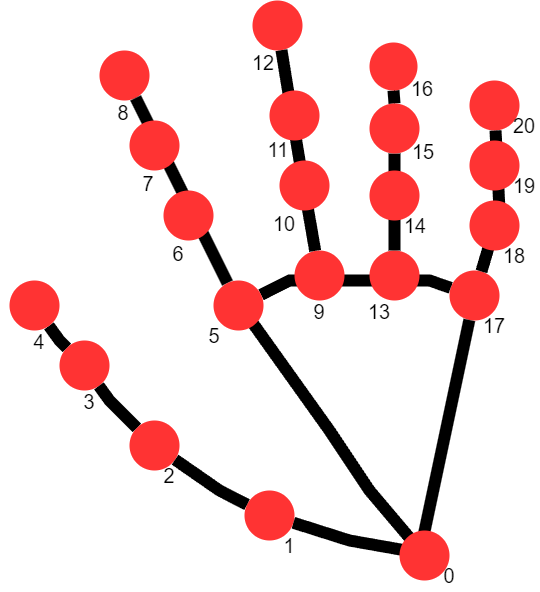
\includegraphics[width=0.5\linewidth]{../Gambar/Handlandmark.png}
	\caption{Dua puluh satu titik \textit{hand landmark} pada tangan}
	\label{fig:tangan}
\end{figure}
Pengenalan gestur atau pose tangan merupakan topik yang menarik dalam ilmu komputer dan teknologi yang betujuan untuk komunikasi antara manusia dengan komputer menggunakan gestur tanpa menyentuhnya secara langsung \parencite{UniversitasDinamika}. Saat ini banyak \textit{framework} atau \textit{library} pembelajaran mesin untuk mengenali gerakan tangan, salah satu yaitu \textit{Mediapipe}. \textit{Mediapipe} merupakan suatu framework yang dirancang oleh Google untuk menghasilkan audio atau video dari membangun \textit{pipelines} untuk mengolah data persepsi. Dengan bantuan dari \textit{Mediapipe} tangan yang terdapat pada citra akan dapat dideteksi dengan mendeteksi dua puluh satu titik pada tangan yang ditunjukkan oleh Gambar \ref*{fig:tangan}. Proses pertama yaitu akan mendeteksi telapak tangan atau disebut \textit{palm detection} agar program dapat mendeteksi keberadaan tangan. Selanjutnya yaitu mendeteksi dua puluh titik \textit{keypoint} dalam tangan yang sudah terdeteksi \parencite{mediapipejurnal}. 


\subsection{\textit{Convolutional Neural Network} (CNN)}
\begin{figure}[!h]
  \centering
  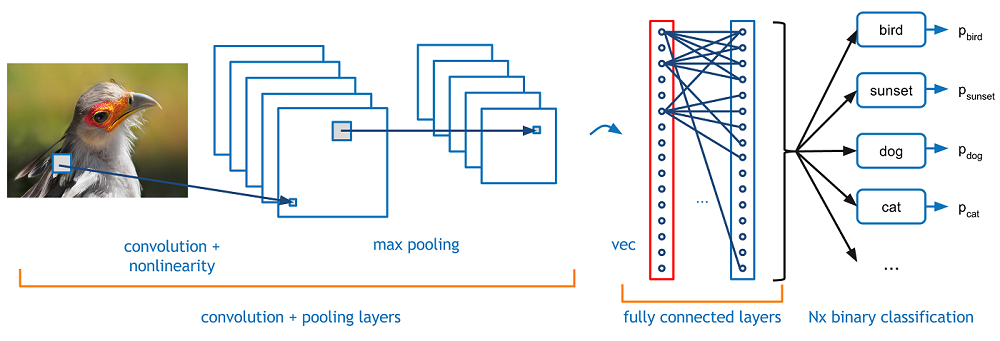
\includegraphics[width=1\linewidth]{../Gambar/cnn.png}
  \caption{Arsitektur CNN \parencite{adit}}
  \label{fig:cnn}
\end{figure}
CNN merupakan salah satu dari \textit{neural network} yang digunakan untuk memproses data berupa grid. Salah satu contoh dari data grid adalah citra. Citra dianggap sebagai grid karena berbentuk piksel dua dimensi. CNN dianggap sebagai salah satu solusi untuk permasalahan pada bidang \textit{Computer Vision} untuk mendeteksi dan mengenali sebuah image \parencite{CNN}. Secara nama CNN menunjukkan bahwa operasi matematika yang akan digunakan yaitu konvolusi dengan cara mengkalikan data dua dimensi dengan kernel. Pada CNN akan memiliki 3 lapisan utama seperti pada Gambar \ref*{fig:cnn} yaitu :
\begin{enumerate}
  \item \textit{Convolutional Layer} \par
  Layer ini merupakan inti dari CNN karena pada layer ini akan dilakukannya operasi konvolusi. Operasi konvolusi pada layer ini akan dilakukan antara input data dengan \textit{filter} atau \textit{kernel}. \textit{Filter} akan melintasi input data dan akan melakukan operasi "dot" antara input data dengan nilai dari \textit{filter} sehingga akan menghasilkan \textit{feature map} \parencite{convolusi}. Proses konvolusi dapat dilihat pada Gambar \ref{fig:konvolusilayer}. 

  \begin{figure}[!h]
    \centering
    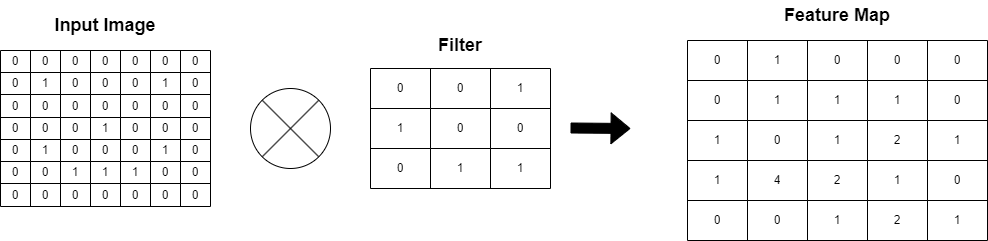
\includegraphics[width=1\linewidth]{../Gambar/konvolusilayer.png}
    \caption{Proses Konvolusi Pada \emph{Convolutional Layer}}
    \label{fig:konvolusilayer}
  \end{figure}
  
  \item \textit{Pooling Layer} \par
  Layer ini digunakan untuk melakukan \textit{downsampling} yang berguna untuk mengurangi dimensi dan jumlah parameter. Terdapat dua jenis \textit{pooling} yang sering digunakan yaitu \textit{max pooling} dan  \textit{average pooling}. \textit{Max pooling} adalah mengambil citra maksimum yang dicakup oleh kernel, sedangkan pada \textit{average pooling} adalah mengambil nilai rata-rata dari citra yang dicakup kernel. Namun tidak hanya itu \textit{pooling layer} juga digunakan untuk mengekstraksi fitur dominan \parencite{Bukusakti}. Pooling yang sering digunakan adalahh \emph{max pooling}. \emph{Max pooling} merupakan proses mengambil nilai terbesar dari sub matriks dan membentuk matriks terpisah. Filter \emph{max pooling} yang sering digunakan berukuran 2x2 yang menyebabkan berkurangnya ukuran input image menjadi setengahnya. Proses \emph{max pooling} dapat dilihat pada Gambar \ref{fig:poolinglayer}

  \begin{figure}[!h]
    \centering
    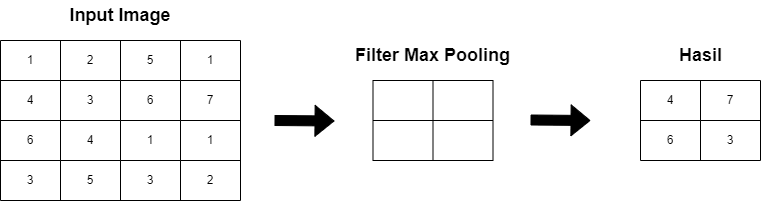
\includegraphics[width=1\linewidth]{../Gambar/maxpooling.png}
    \caption{Proses \emph{Max Pooling} Pada \emph{Pooling Layer}}
    \label{fig:poolinglayer}
  \end{figure}

  \item \textit{Fully Connected Layer} \par
  Layer ini digunakan untuk melakukan transformasi pada dimensi data agar dapat diklasifikasikan secara liner.
  Hasil dari \textit{pooling layer} masih berbentuk \textit{multidimensional array}, maka dari itu pada \textit{fully connected layer} akan dilakukan \textit{reshape} input dari \textit{multidimensional array} menjadi vector. Setiap \textit{neuron} pada \textit{convolutional layer} akan ditransformasikan menjadi data satu dimensi sebelum dapat dimasukkan dalam sebuah \textit{fully connected layer} \parencite{JurnalTeknikITS}.
\end{enumerate} 

\subsection{Matriks Evaluasi}
Matriks evaluasi merupakan matriks yang digunakan dalam evaluasi hasil dalam \emph{machine learning} untuk mengukur model secara statistika. Matriks evaluasi terdapat beberapa jenis yang dapat digunakan sesuai dengan kebutuhan diantaranya seperti \emph{classification accuracy}, \emph{logarithmic loss}, dan \emph{confusion matrix}. Matriks evaluasi yang digunakan pada tugas akhir ini menggunakan \emph{confusion matrix}. Confusion matrix terdapat empat istilah representasi hasil proses klasifikasi yaitu :
\begin{enumerate}
  \item \emph{True Positive}. \par
  \emph{True positive} memiliki arti bahwa suatu model memprediksi data pada kelas positif dan data yang sebenarnya berada pada kelas positif.
  \item \emph{True Negative}. \par
  \emph{True negative} memiliki arti bahwa suatu model memprediksi data pada kelas negatif namun data yang sebenarnya berada pada kelas positif.
  \item \emph{False Positive}. \par
  \emph{False positive} memiliki arti bahwa suatu model memprediksi data pada kelas positif namun data yang sebenarnya berada pada kelas negatif.
  \item \emph{False Negative}. \par
  \emph{False negative} memiliki arti bahwa suatu model memprediksi data pada kelas negatif dan data yang sebenarnya berada pada kelas negatif.
\end{enumerate}

Confusion matrix dapat digunakan untuk mencari nilai Precision, Recall, dan Akurasi dari model yang telah dibuat menggunakan empat istilah dalam confusion matrix. Bentuk confusion matrix dapay dilihat pada Gambar \ref{fig:bentukconfusionmatrix}. 

% Precision adalah suatu nilai yang didapatkan dengan cara membagi jumlah total pada \emph{True Positive} atau jumlah data positif yang diklasifikasikan bernilai benar dengan jumlah total data positif yang diprediksi atau \emph{True Positive} ditambah dengan \emph{False Positive} \parencite{precision}. Recall atau sensitivity merupakan suatu nilai yang didapatkan dengan cara membagi jumlah data positif yang diklasifikasikan bernilai benar dengan jumlah  total data positif. Akurasi merupakan ketepatan pengukuran terhadap nilai sebenarnya \parencite{akurasi}. Perhitungan akurasi didapatkan dari jumlah total data yang diklasifikasikan benar pada class  Persamaan Precision dapat dilihat pada Persamaan \ref{eq:precision} dan persamaan Recall dapat dilihat pada Persamaan \ref{eq:recall}. Nilai akurasi didapatkan dengan menggunakan Persamaan \ref{eq:akurasi}.

\begin{figure}[H]
  \begin{tabular}{|cc|cc|}
    \hline
    \multicolumn{2}{|c|}{\multirow{2}{*}{}}                    & \multicolumn{2}{c|}{Aktual}              \\ \cline{3-4} 
    \multicolumn{2}{|c|}{}                                     & \multicolumn{1}{c|}{Positive} & Negative \\ \hline
    \multicolumn{1}{|c|}{\multirow{2}{*}{Prediksi}} & Positive & \multicolumn{1}{c|}{TP}       & FP       \\ \cline{2-4} 
    \multicolumn{1}{|c|}{}                          & Negative & \multicolumn{1}{c|}{FN}       & TN       \\ \hline
    \end{tabular}
    \centering
    \caption{Bentuk \emph{confusion matrix}}
    \label{fig:bentukconfusionmatrix}
\end{figure}

% \begin{equation}
%   \label{eq:precision}
%   Akurasi = \frac{TP}{TP + FP}
% \end{equation}

% \begin{equation}
%   \label{eq:recall}
%   Akurasi = \frac{TP}{TP + FN}
% \end{equation}

% \begin{equation}
%   \label{eq:akurasi}
%   Akurasi = \frac{TP + TN}{TP + TN + FP + FN}
% \end{equation}

